\documentclass[10pt,aspectratio=169]{beamer}

% All the boilerplate is in ccaslides.sty
% Note that this also pulls in a custom vogtwidebar.sty
\usepackage{ccaslides}

\author{Ji\v{r}\'i Lebl}

\institute[OSU]{%
Departemento pri Matematiko de Oklahoma {\^S}tata Universitato}

\title{Cultivating Complex Analysis:\\%
Wild world of essential singularities, Casorati--Weierstrass (5.2.3)}

\date{}

\begin{document}

\begin{frame}
\titlepage
\end{frame}

\begin{frame}
Consider a ``plot'' of $e^{1/z}$.

\vspace*{-15pt}
\hspace*{2.2in}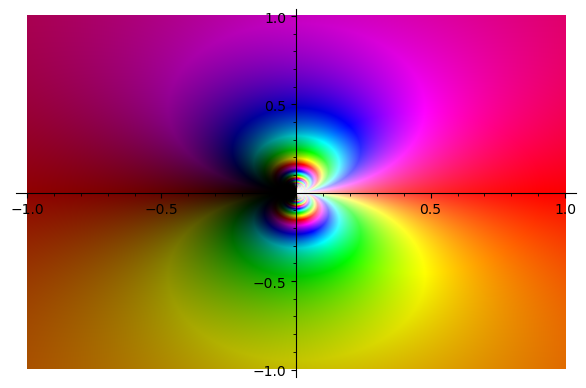
\includegraphics[width=3.5in]{essential-sing.png}

\vspace*{-2.05in}
Values of $e^{1/z}$ are shown using

\medskip
modulus as brightness,

\medskip
argument as hue (color).

\medskip
\pause

It seems like near zero,

we achieve every value.

\medskip
\pause

We actually get $\C \setminus \{ 0 \}$ as

the image of any neighborhood of $0$.

\end{frame}

\begin{frame}
\begin{theorem}[Casorati--Weierstrass]
Suppose $U \subset \C$ is open and $f \colon U \setminus \{ p \} \to \C$ is
holomorphic with
an essential singularity at $p \in U$.
\pause

Then for every punctured disc
$\Delta_r(p) \setminus \{ p \} \subset U$, the image
\begin{equation*}
f\bigl(\Delta_r(p) \setminus \{ p \} \bigr)
=
\bigl\{ w \in \C : w = f(z), \, z \in \Delta_r(p) \setminus \{ p \} \bigr\}
\quad \text{is dense in } \C.
\end{equation*}
\end{theorem}

\pause

Intuitive idea of the proof:

If a whole disc $\Delta_s(q)$ is missing from the image,
take $q$ to $\infty$ by an LFT.

\medskip
\pause

$\Delta_s(q)$ goes to the complement of a bounded closed disc,
and Riemann extension applies.

\pause
\medskip

\textbf{Remark:}
There is a stronger (and much harder to prove) theorem:

\pause
\medskip

Picard's theorem says

$f\bigl(\Delta_r(p) \setminus \{ p \} \bigr) = \C$ or 

$f\bigl(\Delta_r(p) \setminus \{ p \} \bigr) = \C \setminus \{ z_0 \}$ for
some $z_0$.

\end{frame}

\begin{frame}

\textbf{Proof} (of Casorati--Weierstrass)\textbf{:}

Suppose $f \colon U \setminus \{ p \} \to \C$ is holomorphic,
$\Delta_r(p) \subset U$, and $\Delta_s(q)$ is such that

\medskip

$\Delta_s(q) \subset \C \setminus f\bigl(\Delta_r(p) \setminus \{ p \} \bigr)$.

\medskip
\pause

Define $g \colon \Delta_r(p) \setminus \{p\} \to \C$ \quad
by \quad $\displaystyle
g(z) = \frac{1}{f(z) - q}$.

\medskip
\pause

$\sabs{f(z)-q} \geq s$ for $z \in \Delta_r(p) \setminus \{p\}$

\medskip
\pause

$\Rightarrow$ \quad
$\sabs{g(z)} \leq \nicefrac{1}{s}$ for $z \in \Delta_r(p) \setminus \{p\}$

\medskip
\pause
$\Rightarrow$ \quad
$g$ has a removable singularity at $p$ by Riemann extension.

\medskip
\pause

So assume $g$ is defined in $\Delta_r(p)$.

\medskip
\pause

$\displaystyle
f(z) = \frac{1}{g(z)} + q
$
\quad
for $z \in \Delta_r(p) \setminus \{ p \}$.

\medskip
\pause

If $g(p)=0$, \quad $\Rightarrow$ \quad $f$ has a pole at $p$.

\medskip
\pause

If $g(p) \not= 0$, \quad $\Rightarrow$ \quad $f$ has a removable singularity at $p$.

\medskip
\pause

In either case, $f$ does not have an essential singularity at $p$.
\qed

\end{frame}

\begin{frame}
\textbf{Exercise:}
Prove the converse of Casorati--Weierstrass.
Let $U \subset \C$ be open, $p \in U$, and
$f \colon U \setminus \{ p \} \to \C$
holomorphic.
Prove that if $f\bigl(\Delta_r(p) \setminus \{ p \} \bigr)$ is dense in $\C$
for all $r > 0$ such that $\Delta_r(p) \subset U$,
then $f$ has an essential singularity at $p$.

\medskip
\pause

\textbf{Exercise:}
Suppose that $g \colon \Delta_r(p) \setminus \{ p \} \to \C$
has an isolated singularity.  Prove $f(z) = e^{g(z)}$
has either a removable or an essential singularity.

\medskip
\pause

\textbf{Exercise:}
Suppose $f \colon \C \to \C$ is holomorphic and nonconstant.
Prove $f(\C)$ is dense in $\C$.
\pause

Remark: The so-called ``little Picard theorem'' says that $f(\C)$
is actually everything minus possibly one point,
but that is much harder to prove.
\end{frame}

\end{document}
